\section{Datasets}
The experiments in this work utilize three widely recognized image classification benchmarks: CIFAR-10, CIFAR-100, and STL-10. The CIFAR-10 dataset contains 60,000 RGB 32x32 images divided into 10 classes, with 6,000 images per class, offering a balanced benchmark for evaluating basic recognition capabilities. CIFAR-100 shares the same total number of images as CIFAR-10 but includes 100 fine grained classes, each represented by 600 images, thereby introducing greater categorization complexity. STL-10 consists of 130,000 higher resolution 96x96 RGB images across 10 classes. These datasets collectively provide a multi-scale evaluation framework, testing the TinyViT architecture across varying class granularities, data volumes, and image resolutions.

\begin{figure}
    \centering
    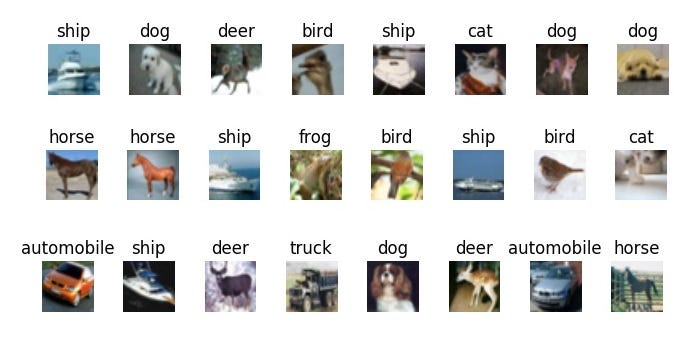
\includegraphics[width=0.5\textwidth]{images/cifar-10.jpg}
    \caption{CIFAR-10 dataset samples images and classes \cite{krizhevsky2009learning}.}
    \label{fig:datasets}
\end{figure}

The experiments uses standard train-test splits for all datasets: CIFAR-10 and CIFAR-100 each include 50,000 training and 10,000 test images, while STL-10 uses 5,000 labeled training images and 8,000 test samples. For CIFAR-10 and CIFAR-100, training data undergoes augmentation via random cropping (32x32 with 4 pixel padding) and horizontal flipping, followed by normalization using channel wise means (0.4914, 0.4822, 0.4465) and standard deviations (0.2470, 0.2435, 0.2616). Test images are directly normalized without augmentation. STL-10, with its higher 96x96 resolution, employs more extensive training augmentations: 12 padded random cropping, horizontal flipping, 15 degree rotations, color jittering (brightness, contrast, saturation), and random grayscaling (10\% probability), normalized with dataset specific statistics (means: 0.4467, 0.4398, 0.4066; stds: 0.2603, 0.2566, 0.2713). Test sets for all datasets apply only resizing, tensor conversion, and identical normalization to ensure evaluation consistency. These transformations balance generalization during training and standardization during testing.